\begin{frame}{\insertsection}

  \begin{columns}
    \begin{column}{.4\textwidth}
      \begin{itemize}[<+-|alert@+>]
      \item Fearlessness
      \item Universality
      \item Combines strengths of ``best tools for the given job''
      \item Ownership system
      \item Community and collaboration
      \item Tooling
      \item Keeps getting better
      \end{itemize}
    \end{column}
    \begin{column}{.6\textwidth}
      \begin{onlyenv}<1>%
        Still have logical problems or wrong architecture, but
        \begin{itemize}
        \item no race conditions,
        \item no leaking resources,
        \item no dangling pointers,
        \item no unhandled exceptions,
        \item no NULL dereferences,
        \item no out of bounds,
        \item ...
        \end{itemize}
        With Rust I can focus on the real problems.
      \end{onlyenv}

      \begin{onlyenv}<2>%
        Rust is reasonably good at pretty much everything.
        \begin{itemize}
        \item Embedded systems
        \item WebAssembly frontend code
        \item Quick and dirty utility
        \item Sophisticated tool
        \item 3D engine or game
        \item Business server-side app
        \item Mobile app
        \item OS and drivers
        \item ...
        \end{itemize}
      \end{onlyenv}

      \begin{onlyenv}<3>%
        \begin{itemize}
        \item The performance, power and control of C/C++
        \item Memory safety of JVM/scripting languages
        \item Expressive type system like OCaml/Haskell/Scala
        \item Automatic memory management like a GC
        \item Dependency management and code sharing like Node
        \item Error messages like Elm
        \item Built-in message passing like Go
        \item ...
        \end{itemize}
      \end{onlyenv}

      \begin{onlyenv}<4>%
        \textit{Bad programmers worry about the code. Good programmers worry
          about data structures and their relationships.}\\[12pt]

        Rust will force you to be a good programmer, you like it or not.
      \end{onlyenv}

      \begin{onlyenv}<5>%
        Rust community is just the best.
      \end{onlyenv}

      \begin{onlyenv}<6>%
        \begin{itemize}
        \item rustup
        \item cargo
        \item xargo
        \item rls
        \item racer
        \item rustfmt
        \item ...
        \end{itemize}
      \end{onlyenv}

      \begin{onlyenv}<7>%
        \center%
        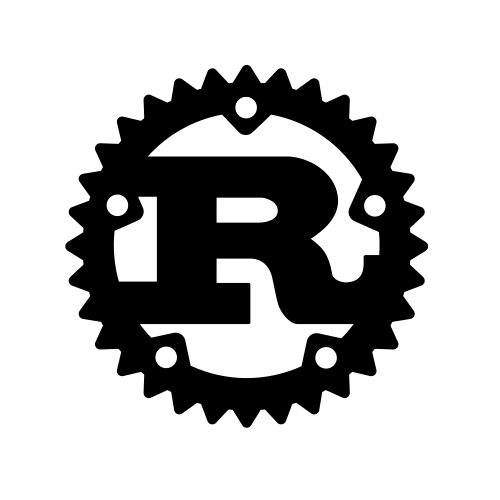
\includegraphics[height = \textheight]{rust_logo.png}%
      \end{onlyenv}
    \end{column}
  \end{columns}

  \note<1>{

    Я практически \textbf{не затронул параллелизм}!

    На Rust легко программировать надёжные системы. Да, я до сих пор буду
    совершать ошибки при разработке системы в целом, но зато мне не надо думать
    о целом классе других ошибок. Я могу полностью сконцентрироваться на
    архитектуре, на конечной цели.

  }

  \note<2>{

    Rust можно использовать для написание практически всего, чего угодно. Я вам
    приводил примеры того, для чего использовал Rust я, а также примеры того,
    где используют Rust крупные компании в production.

  }

  \note<3>{

    Rust объединяет в себе лучшее других языков, при этом оставляет за бортом
    плохое.

    \begin{itemize}
    \item Но безопасный и более юзабельный.
    \item Но без тяжёлого runtime.
    \item Но без GC и его проблем как таковых.
    \item Взято у других и улучшено.
    \end{itemize}

  }

  \note<4>{

    Благодаря системе владения, приходится писать код короче, быстрее, лёгким
    для понимания и изменения, хочу я этого или нет (иначе компилятор будет
    ругаться).

  }

  \note<5>{

    Я реально не встречал сообщества более лучшего, чем у Rust. Вы можете просто
    кинуть ссылку на Playground и попросить сделать code review. И вам его
    сделают, какой бы уровень у вас не был.

    Мейнтейнеры самые доброжелательные, многие пофиксят баги, которые ты
    попросишь, потому что писать на Rust в кайф, хочется, чтобы твой код был
    максимально чистым и рабочим.

  }

  \note<6>{

    Все тулы для Rust кажутся идиоматичными и составляют единое целое. Пока не
    попробуешь --- не поймёшь.

  }

  \note<7>{

    Что ни новая версия Rust --- то стабилизация какой-то крутой фичи. Многие
    языки программирования копируют концепции Rust.

    Заинтересовавшимся \textbf{могу накидать кучу ссылок}, где Rust описывается
    профессиональными разработчиками на C/C++, а также где Rust приходит на
    замену чего-либо (C/C++ или Python).

  }

\end{frame}

\begin{frame}[standout]
  \color{dWhite}Questions?
\end{frame}